\usetikzlibrary{calc,arrows.meta,patterns,angles,quotes}
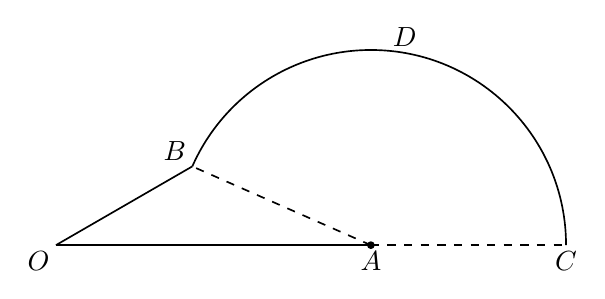
\begin{tikzpicture}[x=1cm,y=1cm,line width=.6pt,font=\normalsize,>=Stealth]
\coordinate (O) at (0.0000000000,0.0000000000);
\coordinate (A) at (4.0000000000,0.0000000000);
\coordinate (B) at (1.7320508076,1.0000000000);
\coordinate (C) at (6.4786273499,0.0000000000);
\coordinate (D) at (4.4304091224,2.4409714310);
\draw (O)--(B);
\draw (O)--(A);
\draw[dashed] (A)--(B);
\draw[dashed] (A)--(C);
\draw (6.4786273499,0.0000000000) arc[start angle=0.0000000000,end angle=156.2060231130,radius=2.4786273499cm];
\node[below left=2pt,inner sep=0pt] at (O) {$O$};
\node[below=2pt,inner sep=0pt] at (A) {$A$};
\node[above left=2pt,inner sep=0pt] at (B) {$B$};
\node[below=2pt,inner sep=0pt] at (C) {$C$};
\node[above=2pt,inner sep=0pt] at (D) {$D$};
\fill (A) circle[radius=1.4pt];
\end{tikzpicture}
